\chapter{System Design} \label{ch:design}
The full system includes a VNA, a turntable, two directional antennas and a computer. This chapter describes the interfaces between the individual parts and their functionalities. In order to get an overview of the full system consider figure \ref{fig:system_design}.
\begin{figure}[H]
    \centering
    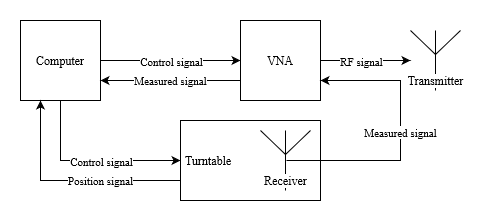
\includegraphics[width=0.8\textwidth]{figures/system_design.png}
    \caption{Overview of system design.} \label{fig:system_design}
\end{figure}
The system is composed of three integrated modules and two directional antennas. The first antenna is a transmitter antenna and the second antenna is a receiver antenna meant to rotate and measure gainm in different directions. These different directions are determined by the turning of the turntable on which the receiver antenna is mounted. Both the transmitter antenna and receiver antenna are connected to a VNA, but for the transmitter antenna, the functionality of the VNA used is the RF generator. For the receiver antenna, the received signal measured by the VNA is then further sent to the computer for data analysis. The computer controls the turntable and the VNA. This includes defining settings before the analysis and taking decisions based on the returned data; the position of the turntable and the measured antenna signal from the VNA. 

% --------------------------------------------------------------------------

\section{Antenna Design} \label{s:ant_design}
The most important characteristics of the antenna chosen for the design is that it is directional. The antenna must be directional in order to detect the direction of transmission. The receiver and transmitter antenna must have the same polarization to ensure that this does not introduce loss in the system. The receiver antenna and the transmitter antenna are chosen to be the same type of antenna with the exact same shape for convenience. This means that all antenna parameters are the same. 

The chosen antenna is a homemade, pyramidal horn antenna. It has a rectangle cross-section, straight curvature of the side walls and therefore a linear polarization. The size of the antenna is \SI{10}{\centi\meter} by \SI{7.65}{\centi\meter} giving an aperture area of \SI{0.00765}{\meter\squared}. The remaining measurements of the sides can be seen on figure \ref{fig:horn_design} on the right and a picture of the antenna on its mount on the left.

\begin{figure}[H]
    \begin{minipage}{0.35\textwidth}
        \centering
        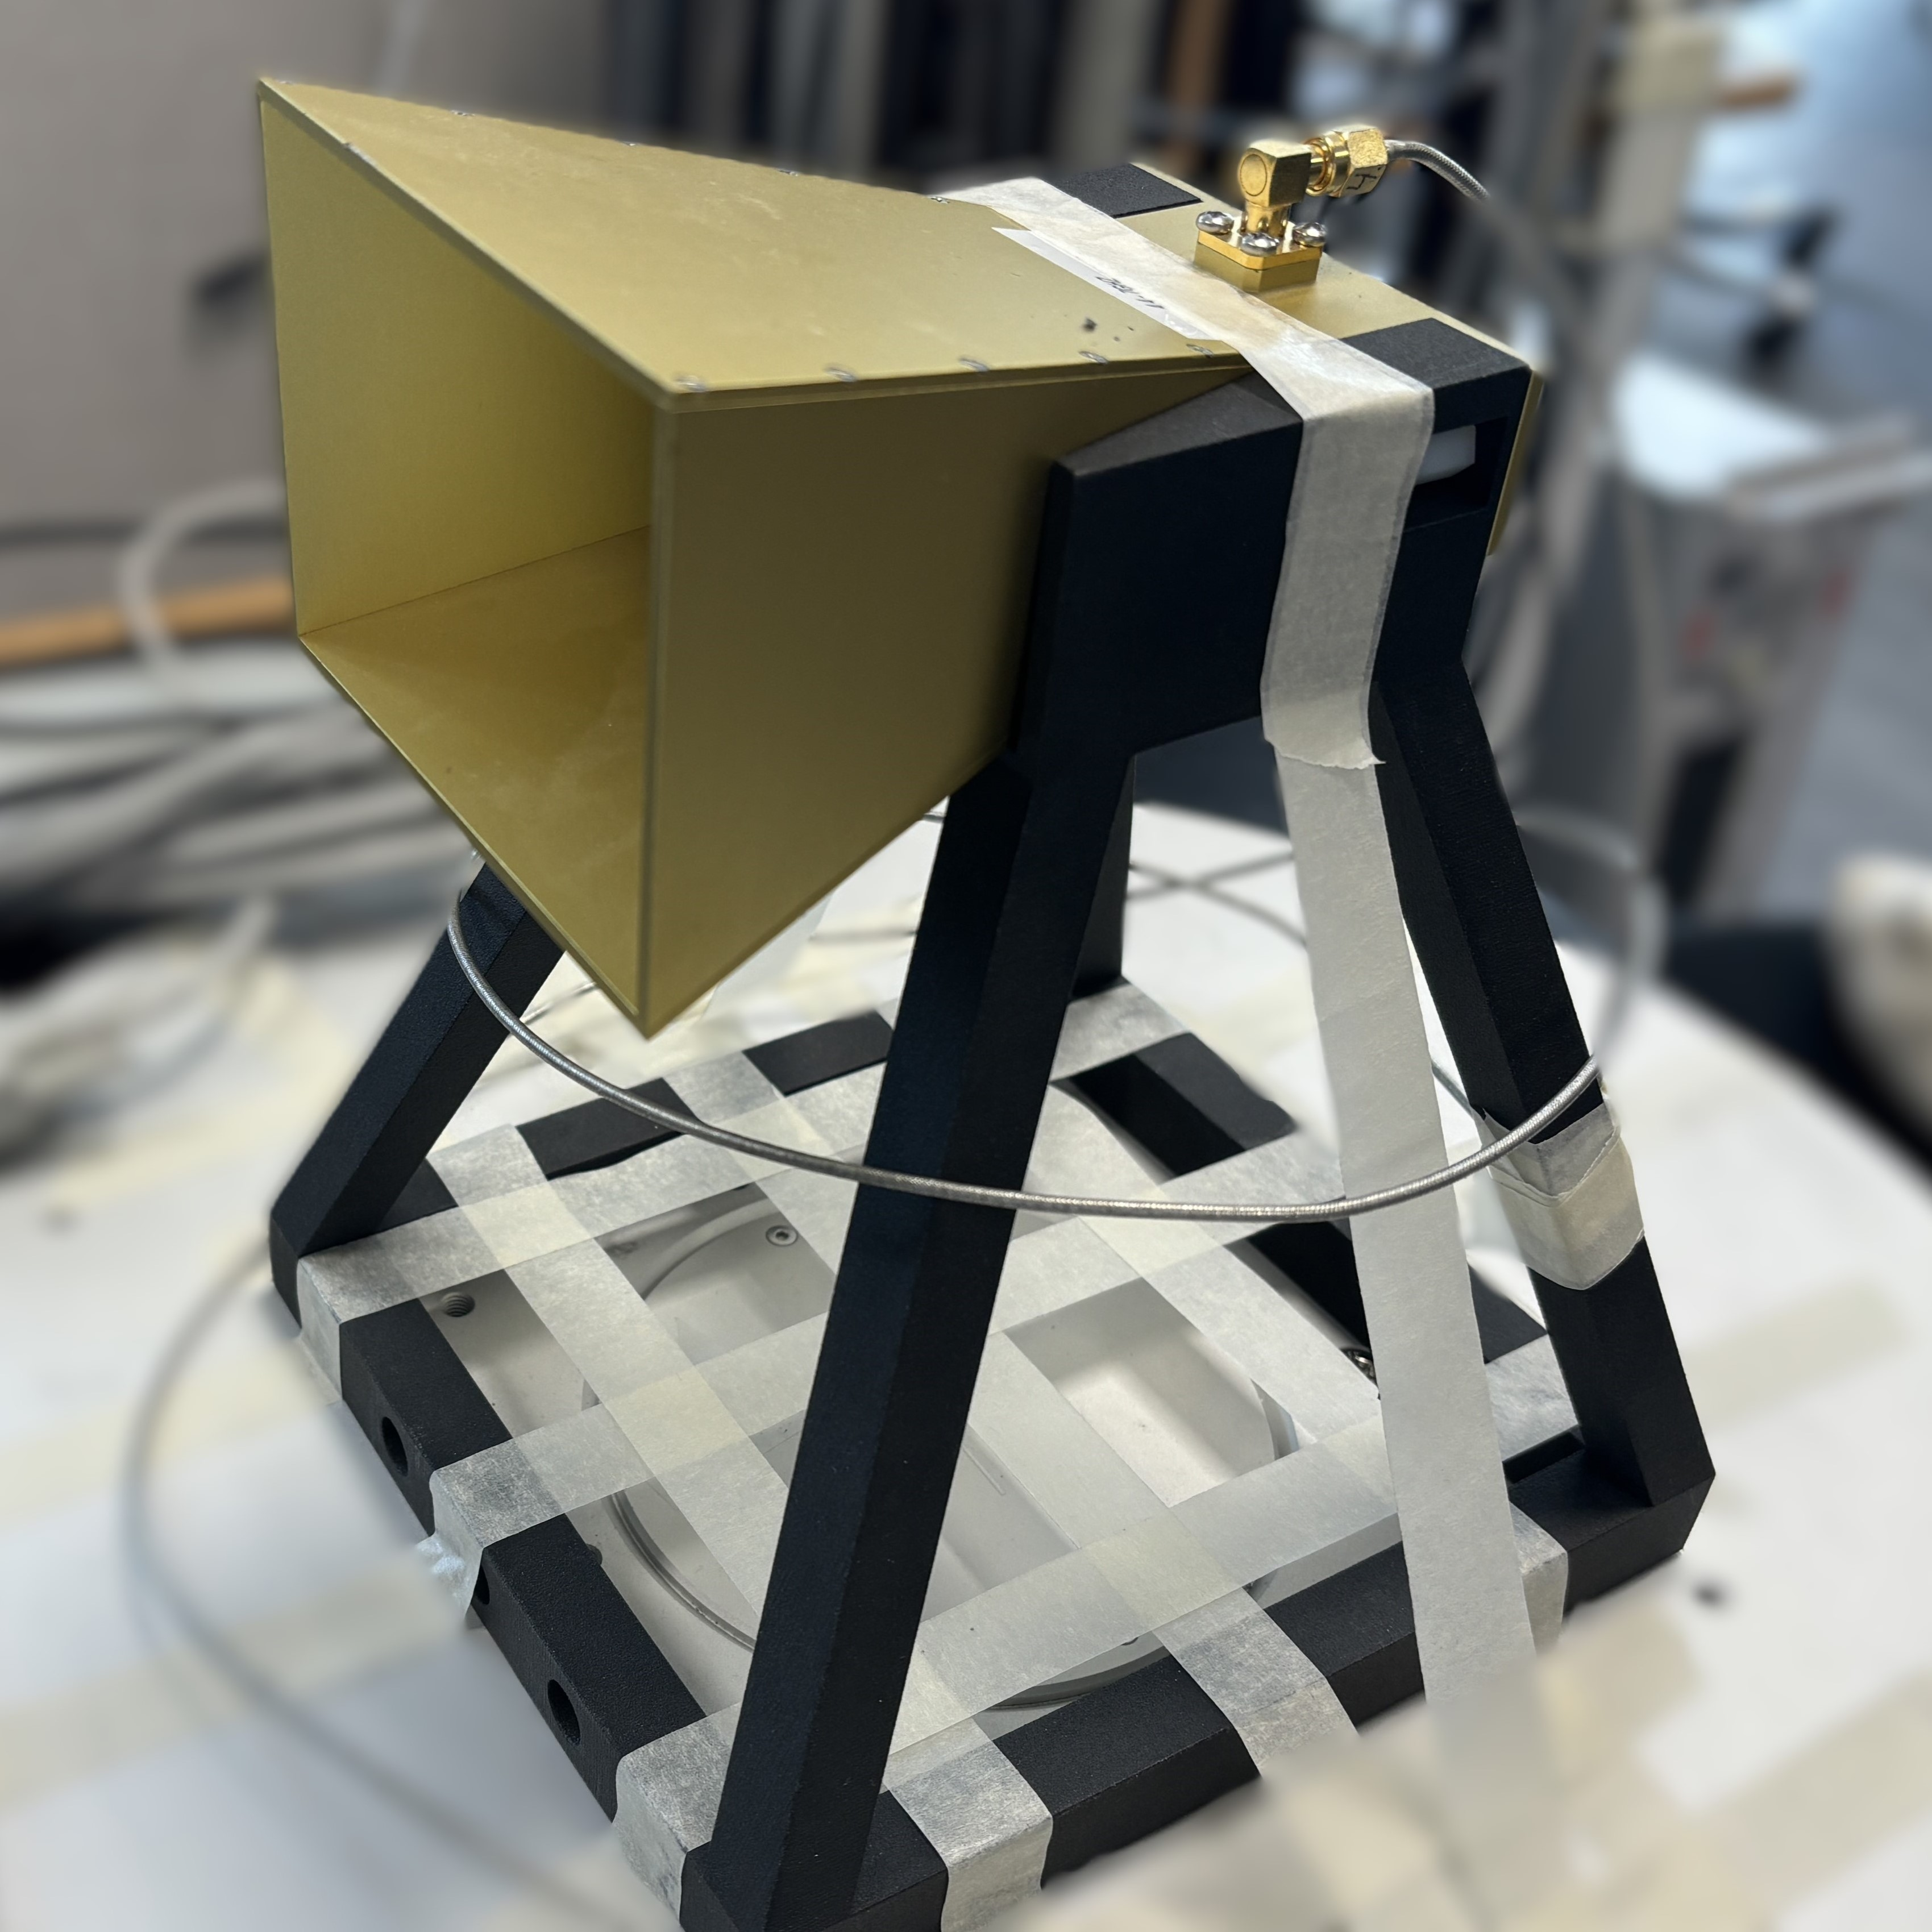
\includegraphics[width=0.9\textwidth]{figures/IMG_2430.JPEG} % first figure itself
    \end{minipage}\hfill
    \begin{minipage}{0.6\textwidth}
        \centering
        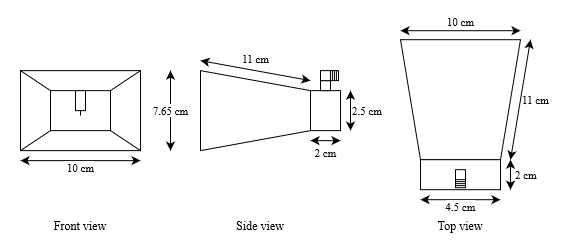
\includegraphics[width=0.9\textwidth]{figures/horn_diagram.png} % second figure itself
    \end{minipage}
    \caption{Horn antenna. Picture and diagram with measurements of horn antenna (not to scale).}
    \label{fig:horn_design}
\end{figure}

In section \ref{ss:friis} the effective aperture of an antenna is given in equation \ref{eq:effectivate_area}. Rewriting this equation to isolate the gain of the receiver antenna in dB gives
\begin{equation} \label{eq:max_gain}
    G_{r,dBi} = 10 \log_{10}\left( \frac{4 \pi}{\lambda^2} A_r \right)
    \tagaddtext{[\si{\decibel}]}
\end{equation}
The frequencies used for testing the system, \SI{4.75}{\giga\hertz} and \SI{5.65}{\giga\hertz}, have been chosen from the test results of S-parameter test in section \ref{s:sparam_test}. The maximum theoretical gains at \SI{4.75}{\giga\hertz} and \SI{5.65}{\giga\hertz}, in the case of the maximum aperture efficiency of 1, are
\begin{equation} \label{eq:max_gain_475}
    G_{r,dBi,4.75} = 10 \log_{10}\left( \frac{4 \pi}{\left(\frac{300E6}{4.75E9}\right)^2} 0.00765 \right) = 13.82
    \tagaddtext{[\si{\decibel}]}
\end{equation}
\begin{equation} \label{eq:max_gain_565}
    G_{r,dBi,5.65} = 10 \log_{10}\left( \frac{4 \pi}{\left(\frac{300E6}{5.65E9}\right)^2} 0.00765 \right) = 15.33
    \tagaddtext{[\si{\decibel}]}
\end{equation}

The antenna has been tested as seen in section \ref{s:sparam_test} and \ref{s:rad_test} to find the return loss $S_{11}$ and the radiation pattern. The horn antenna has a $S_{11}$ magnitude of \SI{-15.71}{\decibel} at \SI{4.75}{\giga\hertz} and \SI{-19.56}{\decibel} at \SI{5.65}{\giga\hertz}. The radiation pattern in the elevation and azimuth planes can be seen in figure \ref{fig:horn_elevation} and figure \ref{fig:horn_azimuth}. The horn antenna has \SI{3}{\decibel}-bandwidths at \SI{22.5}{\degree} for $f=\SI{4.75}{\giga\hertz}$ and at \SI{19}{\degree} for $f=\SI{5.65}{\giga\hertz}$.

% --------------------------------------------------------------------------

\section{Choice of Turntable}
The turntable must be able to be remotely controlled and precise, so that the angular position of the antenna can be determined confidently. The turntable must be able to turn to a remotely specified angle at each turn. 

The \textit{Head Acoustics, HRT I} turntable was available and fulfills the requirements. It has the ability to turn \SI{360}{\degree} with angle steps of \SI{0.1}{\degree}. It can be manually controlled and remotely controlled with software tools. It is able to turn at a maximum speed of \SI{2}{rpm} by a step motor~\cite{hrt_i_data_sheet}. 


% --------------------------------------------------------------------------

\section{Choice of Vector Network Analyzer}
The VNA must have a minimum of two ports, one for input and one for output, be able to be calibrated to normalize the transmission lines to the antennas and must be able to be remotely controlled. Moreover, it must cover the frequency range of the horn antennas. The \textit{Rohde \& Schwarz ZVB8} covers the range from \SI{300}{\kilo\hertz} to \SI{8}{\giga\hertz} with \SI{1}{\hertz} resolution. It can have a measurement time of $<\SI{4.5}{\milli\second}$ with simultaneous data transfer, which allows for fast execution of measurements. The internal noise level is frequency dependent and maximum $<-\SI{70}{dBm}$~\cite[p. 14]{vna_data_sheet_spec}.


% --------------------------------------------------------------------------

\section{Design of Software Control Program}
Using a computer for the control of every aspect of the system allows for the devices to be programmed to operate concurrently. Both the VNA and the turntable are able to be controlled in \textit{Python}. The control of the turntable is implemented as adviced by the manual (see \cite{hrt_i_manual}) with the supplied software \textit{RC-HRT I}. In order to control the turntable, the \textit{RC-HRT I} software is interfaced via the \textit{Python} module \textit{pywin32}, which provides access to the Windows APIs~\cite{pywin32}. \textit{Rohde \& Schwarz} have published a \textit{Python} module for control of the VNA. The \textit{Rohde \& Schwarz} module adds an API for the remote control of the VNA, which is communicated with over TCP using SCPI-commands \textit{(Standard Commands for Programmable Instruments)}. Finally, thread parallelism is achieved with the module \textit{threading}, which is what allows for the design of the control flow to work more efficiently by creating a thread for each device.


% --------------------------------------------------------------------------

\subsection{Communication Interfaces} \label{ss:com_interface}
The communication interfaces of the program is limited by the choice of the VNA and the turntable. The \textit{HEAD Acoustics, HRT I} turntable that has been chosen can be controlled by serial communication using the RS485-standard~\cite{hrt_i_data_sheet}. However, it can also be controlled by its accompanying Windows driver and software control program that accesses the Windows APIs. This requires the Windows registry to be updated with the UUID found in the control interface manual. With the Windows APIs accessible, the turntable can be controlled with predefined methods defined in the operating manual~\cite{hrt_control_api_manual}. 

The \textit{Rohde \& Schwarz ZVB8} VNA has a LAN type interface for control and data transfer~\cite[p. 5.3]{vna_data_sheet_spec}. LAN allows for mutual communication between devices. LAN covers both the physical layer in the form of cabling and network cards, the latter which also contains part of the link layer in the form of logic decisions, and the link layer which includes the link protocol~\cite[p. 153]{tcp_ip}. In order to communicate across a LAN the computers must be connected to the same network and know each other's addresses~\cite[p. 174-175]{tcp_ip}. TCP ensures a connection between the two applications running on the computer and the VNA by a port number. Moreover, the TCP header includes an acknowledgement number which the applications use to acknowledge to each other, that the previous message was correctly received~\cite[p. 313]{tcp_ip}. The content of the TCP packets is SCPI commands and device-specific commands that follow the SCPI-standard~\cite[p. 5.4]{vna_data_sheet_spec}.

% --------------------------------------------------------------------------

\subsection{Concurrency}
Because communication with the turntable and the turning process and communication with the VNA are both I/O bound tasks, there is a risk of wait time. Therefore, in order to achieve concurrent communication and data processing, the wait time is exploited by use of the Python module \textit{threading}. \textit{Threading} uses a single processor and pre-emptive multitasking to acheive concurrency~\cite{concurrency}. This means that at any time if one thread is not using CPU computation the processor can switch to another thread and continue computation here. The processor also saves the current state of each thread so that it can return to the exact same place. This also means that reading and writing to global variables must be protected, because the processor can switch in the middle of a read/write statement. Likewise, if a thread needs to wait for another thread to execute a specific task, it is necessary that the user defines a wait flag, which synchronises the wait between relevant threads~\cite{concurrency}. The \textit{threading} module implements no option to set thread priorities or make scheduling principles~\cite{threading}.

% Have viden om teorier og metoder til spektralestimering. 
% HVILKET BETYDER:
% Anvende relevante værktøjer som f.eks. Matlab eller Python til spektralestimering.
% Teori og metoder til non-parametrisk spektralestimering, herunder f.eks. Diskret Fourier Transformation (DFT) og dennes realisation i form af Fast Fourier Transformation (FFT) og Short Time Fourier Transformation (STFT).
% Kunne anvende relevante softwareværktøjer til at simulere ovenstående systemer.
% Have kendskab til forskellige metoder til at designe analoge og digitale filtre
% Kunne anvende Fouriertransformationen til at analysere digitale signaler.
% Kunne anvende feedback til at reducere påvirkningen af forstyrrelser, usikkerheder etc. samt kunne opstille krav til en ønsket systemrespons for lineære systemer og opnå denne.
% kunne forstå realtidsaspekter i forhold til digitale systemer der kommunikerer med andre analoge og/eller digitale systemer.

% Kunne forstå digitale og analoge overføringsfunktioner beskrevet via hhv. z-operatoren og Laplace-operatoren, herunder elementer som poler, nulpunkter, analoge og digitale implementeringer, overføringsfunktionsmatricer etc.
% kunne linearisere ikke-lineære systemmodeller med henblik på at approksimere dem med lineære modeller.
% Kunne anvende metoder til at modellere fysiske systemer, herunder elektriske, elektromekaniske, termiske og hydrodynamiske systemer, på et niveau hvor modellerne kan bruges i designet af elektroniske systemer der interagerer med deres omgivelser.
% Have viden om OSI netværksmodellen.
% Have viden om protokoller i forskellige lag i systemer der kommunikerer med andre systemer.

%In order to prevent aliasing the alias-free range must be calculated. As described in section \ref{sss:aliasing} the range depends on the settings on the network analyzer. The frequency span together with the number of points also affect how fast each measurement of the entire span can be made. 
%\todo[inline, color=red]{describe what happens with each setting + what sweep frequency(?) does}
%The frequency span is chosen from \SI{5}{\giga\hertz} to \SI{7}{\giga\hertz} which is most of the range of which the horn antenna is designed to work in. The number of points is chosen to be \SI{1001}{} because lowering this value by a couple factors will affect the measurement speed negatively. Therefore the alias-free range is
%\begin{equation}
%    Range = \frac{1001-1}{\SI{5E9}{\hertz}-\SI{7E9}{\hertz}} \SI{300E6}{\meter\per\second} = 150
%    \tagaddtext{[\si{\meter}]}
%\end{equation}